%PREAMBULO
\usepackage{pgfplots}

%CUERPO
\begin{document}
    Ejercicio 2. La puntuación obtenida por 50 personas que se presentaron a una prueba de selección, sumadas las puntuaciones de los distintos tests fueron: 
    \\
    \\
    174, 185, 166, 176, 145, 166, 191, 175, 158, 156, 156, 187, 162, 172, 197, 181, 151,
    161, 183, 172, 162, 147, 178, 176, 141, 170, 171, 158, 184, 173, 169, 162, 172, 181,
    187, 177, 164, 171, 193, 183, 173, 179, 188, 179, 188, 179, 167, 178, 180, 168, 148, 173.
    \\
    \\
    POBLACIÓN: Las personas que se presentaron a la prueba de selección\\
    TAMAÑO: 50\\
    MODALIDADES: Los intervalos que contienen las notas que han obtenido las personas en la prueba
    
    \vspace{5mm}
    a) Agrupar los datos en intervalos de amplitud 5 desde 140 a 200 y dar la tabla de frecuencias.
    \\
    \begin{center}
    \begin{tabular}{| c | c | c | c | c |}
        \hline
        $x_i$ & $n_i$ & $N_i$ & $f_i$ & $F_i$ \\ \hline
        (140-145] & 2 & 2 & 0,04 & 0,04 \\
        (145-150] & 2 & 4 & 0,04 & 0,08 \\
        (150-155] & 1 & 5 & 0,02 & 0,1 \\
        (155-160] & 4 & 9 & 0,08 & 0,18 \\
        (160-165] & 5 & 14 & 0,1 & 0,28 \\
        (165-170] & 6 & 20 & 0,12 & 0,4 \\
        (170-175] & 10 & 30 & 0,2 & 0,6 \\
        (175-180] & 8 & 38 & 0,16 & 0,76 \\
        (180-185] & 6 & 44 & 0,12 & 0,88 \\
        (185-190] & 3 & 47 & 0,06 & 0,94 \\
        (190-195] & 2 & 49 & 0,04 & 0,98 \\
        (195-200] & 1 & 50 & 0,02 & 1 \\
        \hline
    \end{tabular} 
    \end{center}
    
    \vspace{5mm}
    
    Establecemos los intervalos de amplitud 5, empezando con 140 y terminando con 200. Para cada intervalo, contamos cuantas personas han obtenido una puntuación que esté dentro de dicho intervalo. Estas son las frecuencias absolutas ($n_i$). 
    Para la frecuencia absoluta acumulada ($N_i$), sumamos la frecuencia absoluta de la modalidad que estamos analizando a la frecuencia absoluta acumulada de la modalidad anterior. O lo que es lo mismo, sumamos las frecuencias absolutas de todas las modalidades hasta la que estamos analizando: $N_i=n_1 + n_2 + ... + n_i$. 
    Para frecuencia relativa, dividimos cada $n_i$ entre n, es decir, entre $N_{12}$, la frecuencia absoluta acumulada de la última modalidad. 
    Para la frecuencia relativa acumulada hacemos lo mismo que para la absoluta acumulada pero con la frecuencia relativa: sumamos las frecuencias relativas de todas las modalidades hasta la que estamos analizando: $F_i=f_1 + f_2 + ... + f_i$. 
    
    \vspace{10mm}
    b) Representar la distribución mediante un histograma, poligonal de frecuencias y curva de distribución.
    
    \begin{center}
    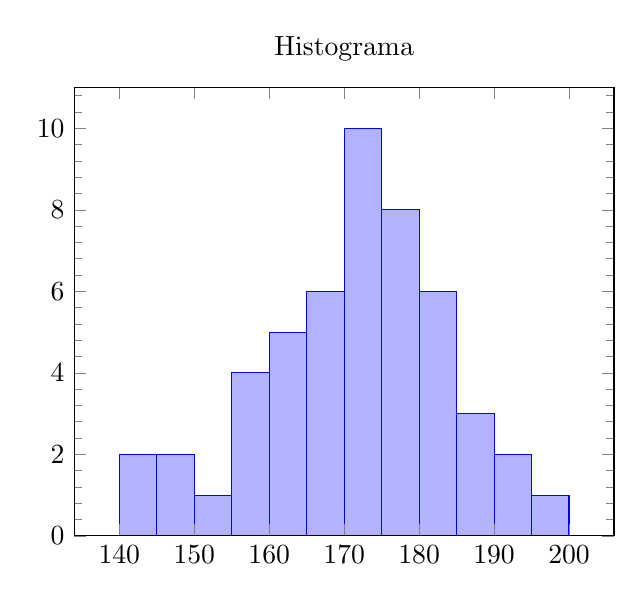
\begin{tikzpicture}
        \begin{axis}[
            title={Histograma},
            ymin=0, ymax=11,
            minor y tick num = 4,
            area style,
            ]
        \addplot+[ybar interval,mark=no] plot coordinates { (140, 2) (145, 2) (150, 1) (155, 4) (160, 5) (165, 6) (170, 10) (175, 8) (180, 6) (185, 3) (190, 2) (195, 1) (200, 0) };
        \end{axis}
    \end{tikzpicture}
    \end{center}
    
    Para el histograma, en el eje x tenemos las modalidades ($x_i$) y en el eje y un múltiplo de hi ($hi=\frac{fi}{a}$). En este caso, las amplitudes de todos los intervalos son iguales: 5. 
    
    \vspace{5mm}
    \begin{center}
    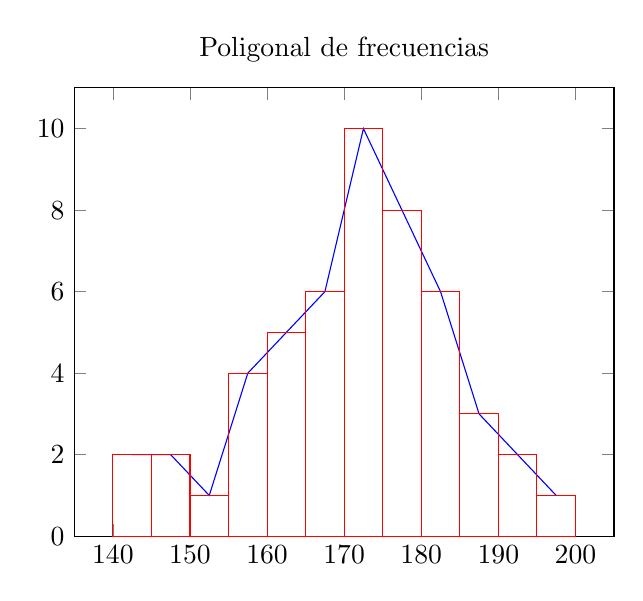
\begin{tikzpicture}
    \begin{axis}[
        title={Poligonal de frecuencias},
        xmin=135, xmax=205,
        ymin=0, ymax=11,
        xtick={140,150,160,170,180,190,200},
        ytick={0,2,4,6,8,10},
        legend pos=north west,
        ymajorgrids=false,
        grid style=dashed,
    ]

    \addplot[
        color=blue,
        ]
        coordinates {
        (142.5,2)(147.5,2)(152.5,1)(157.5,4)(162.5,5)(167.5,6)(172.5,10)(177.5,8)(182.5,6)(187.5,3)(192.5,2)(197.5,1)
        };
            [
            ymin=0, ymax=11,
            minor y tick num = 4,
            area style,
            ]
        \addplot+[ybar interval,mark=no] plot coordinates { (140, 2) (145, 2) (150, 1) (155, 4) (160, 5) (165, 6) (170, 10) (175, 8) (180, 6) (185, 3) (190, 2) (195, 1) (200, 0) };
    
    \end{axis}
    \end{tikzpicture}
    \end{center}
    
    Para el poligonal de frecuencias, los ejes son los mismos que para el histograma. En este caso, unimos los puntos que corresponden a las marcas de los intervalos en el histograma. Para hallar las marcas de los intervalos: $c_i=\frac{e_{i-1}+e_i}{2}$.
    
    \begin{center}
    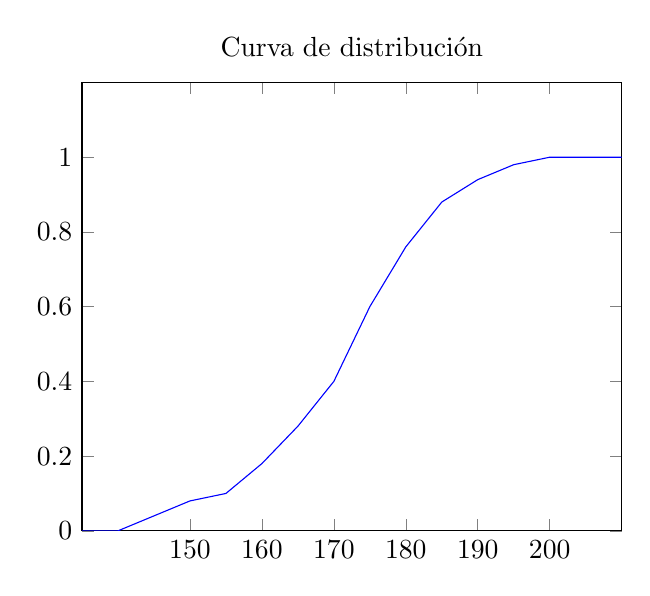
\begin{tikzpicture}
    \begin{axis}[
        title={Curva de distribución},
        xmin=135, xmax=210,
        ymin=0, ymax=1.2,
        xtick={150,160,170,180,190,200},
        ytick={0,0.2,0.4,0.6,0.8,1},
        legend pos=north west,
        ymajorgrids=false,
        grid style=dashed,
    ]

    \addplot[
        color=blue,
        ]
        coordinates {
        (135,0)(140,0)(145,0.04)(150,0.08)(155,0.1)(160,0.18)(165,0.28)(170,0.4)(175,0.6)(180,0.76)(185,0.88)(190,0.94)(195,0.98)(200,1)(205,1)(210,1)
        };
    
    \end{axis}
    \end{tikzpicture}
    \end{center}
    
    En la curva de distribución, en el eje x tenemos los extremos superiores de los intervalos $(e_i)$ y en el eje y, $F(e_i)$. Pintamos la curva que une los puntos tal que $F(e_i)=\displaystyle\sum_{j=1}^{i}f_{j}=F_i$. En este caso tenemos que la curva es continua. $F(e_i)$ es 0 para valores menores que $e_1$ y 1 para valores mayores que el último intervalo $e_k$.
    
\end{document}
